\documentclass[notes=only]{beamer}

\usepackage{tikz}
\usetheme{Berlin}
\usecolortheme{beaver}

\usepackage[main=russian,english]{babel} 
\usepackage[]{graphicx} 
\graphicspath{{images/}}
\usepackage[]{booktabs}

%Содержание в начале секций
\AtBeginSection[]
{%
  \begin{frame}
    \tableofcontents[currentsection]
  \end{frame}
}

%Титульный лист
\title[тактильные шахматы]{ТАКТИЛЬНЫЕ ШАХМАТЫ}
\subtitle{проектная работа}
\author{Максимов Матвей}
\institute[МБОУ СОШ №73]{%
    Муниципальное бюджетное общеобразовательное учреждение\\
    <<Средняя общеобразовательная школа №73>>\\
    11 А класс}
\date{Февраль 2023 г.}

\begin{document}
\frame{\titlepage}

\section{Введение}

\begin{frame}
    \frametitle{Тема работы}
    \begin{center}
        Специализированные шахматы для слабовидящих людей
    \end{center}
\end{frame}

\begin{frame}
    \frametitle{Актуальность темы проекта}
    По данным статистики, в России слабовидящими и слепыми людьми признаны
    более 210'000 человек. Это население среднего российского города. Многие из
    этих людей не могут сыграть в шахматы из-за высокой стоимости шахматного
    набора для слабовидящих людей или не знания о существовании шахмат,
    специализированных для слабовидящих людей. Это актуализирует проблему малой
    доступности шахмат для слабовидящих людей и о организациях, подобных IBCA\@.
\end{frame}

\begin{frame}
    \frametitle{Цель работы}
    \begin{enumerate}
        \item Проанализировать исторические прототипы и современные аналоги
        \item Предложить решение выявленных проблем
        \item Реализовать предложенные методы решения
    \end{enumerate}
\end{frame}

\begin{frame}
    \frametitle{Задачи}
    \begin{enumerate}
        \item Разработать тактильные шахматы для слабовидящих людей
        \item Разработать метод, позволяющий расширить аудиторию, осведомлённую
            о существовании специализированных шахмат для слабовидящих людей
    \end{enumerate}
\end{frame}

\section{Теоретический этап}

\begin{frame}
    \frametitle{Стандартизованная шахматная доска}
    \begin{figure}[htpb]
        \centering
        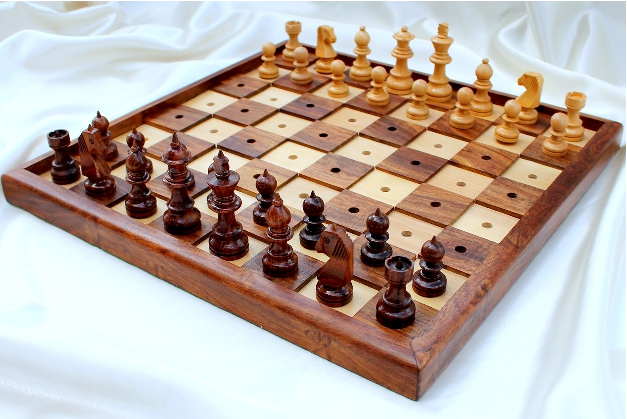
\includegraphics[width=0.8\textwidth]{blind-chess}
    \end{figure}
\end{frame}
\note{%
    Шахматная доска, используемая слабовидящими игроками сконструирована
    следующим образом:
    \begin{enumerate}
        \item Все чёрные квадраты возвышаются на 3--4 мм над белыми.
        \item Каждый из квадратов на доске имеет отверстие в центре, чтобы
            шахматные фигуры могли быть закреплены в этих отверстиях.
        \item Каждая фигура имеет в основании направленный вниз выступ
            (гвоздь), который входит в отверстие в квадратах на доске.
        \item На верхушках всех чёрных фигур закреплена булавка, помогающая
            игроку различать белые и чёрные фигуры.
    \end{enumerate}
}

\begin{frame}
    \frametitle{Критерии к изделию}
    \begin{enumerate}
        \item возможность быстро ощупать большое число фигур
        \item сложность случайно сдвинуть или уронить фигуру
        \item возможность легко и быстро нащупать границы поля на доске
        \item удобство во время игры
        \item удобство при складывании и раскладывании фигур и доски
        \item простота и низкая стоимость изготовления
    \end{enumerate}
\end{frame}

\begin{frame}
    \frametitle{Азиатские аналоги шахмат}
    \begin{columns}
        \column{0.5\textwidth}
        \begin{figure}[htpb]
            \centering
            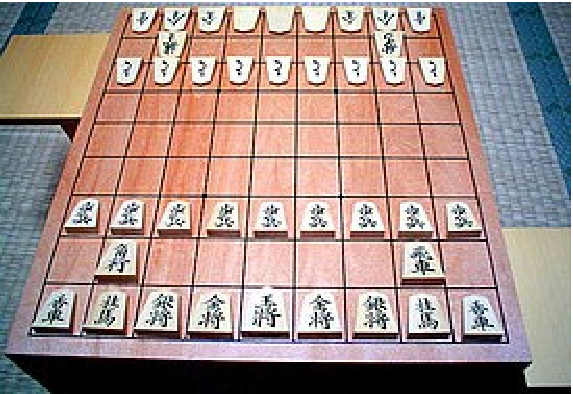
\includegraphics[width=0.7\textheight]{shogi}
            Сёги
        \end{figure}

        \column{0.5\textwidth}
        \begin{figure}[htpb]
            \centering
            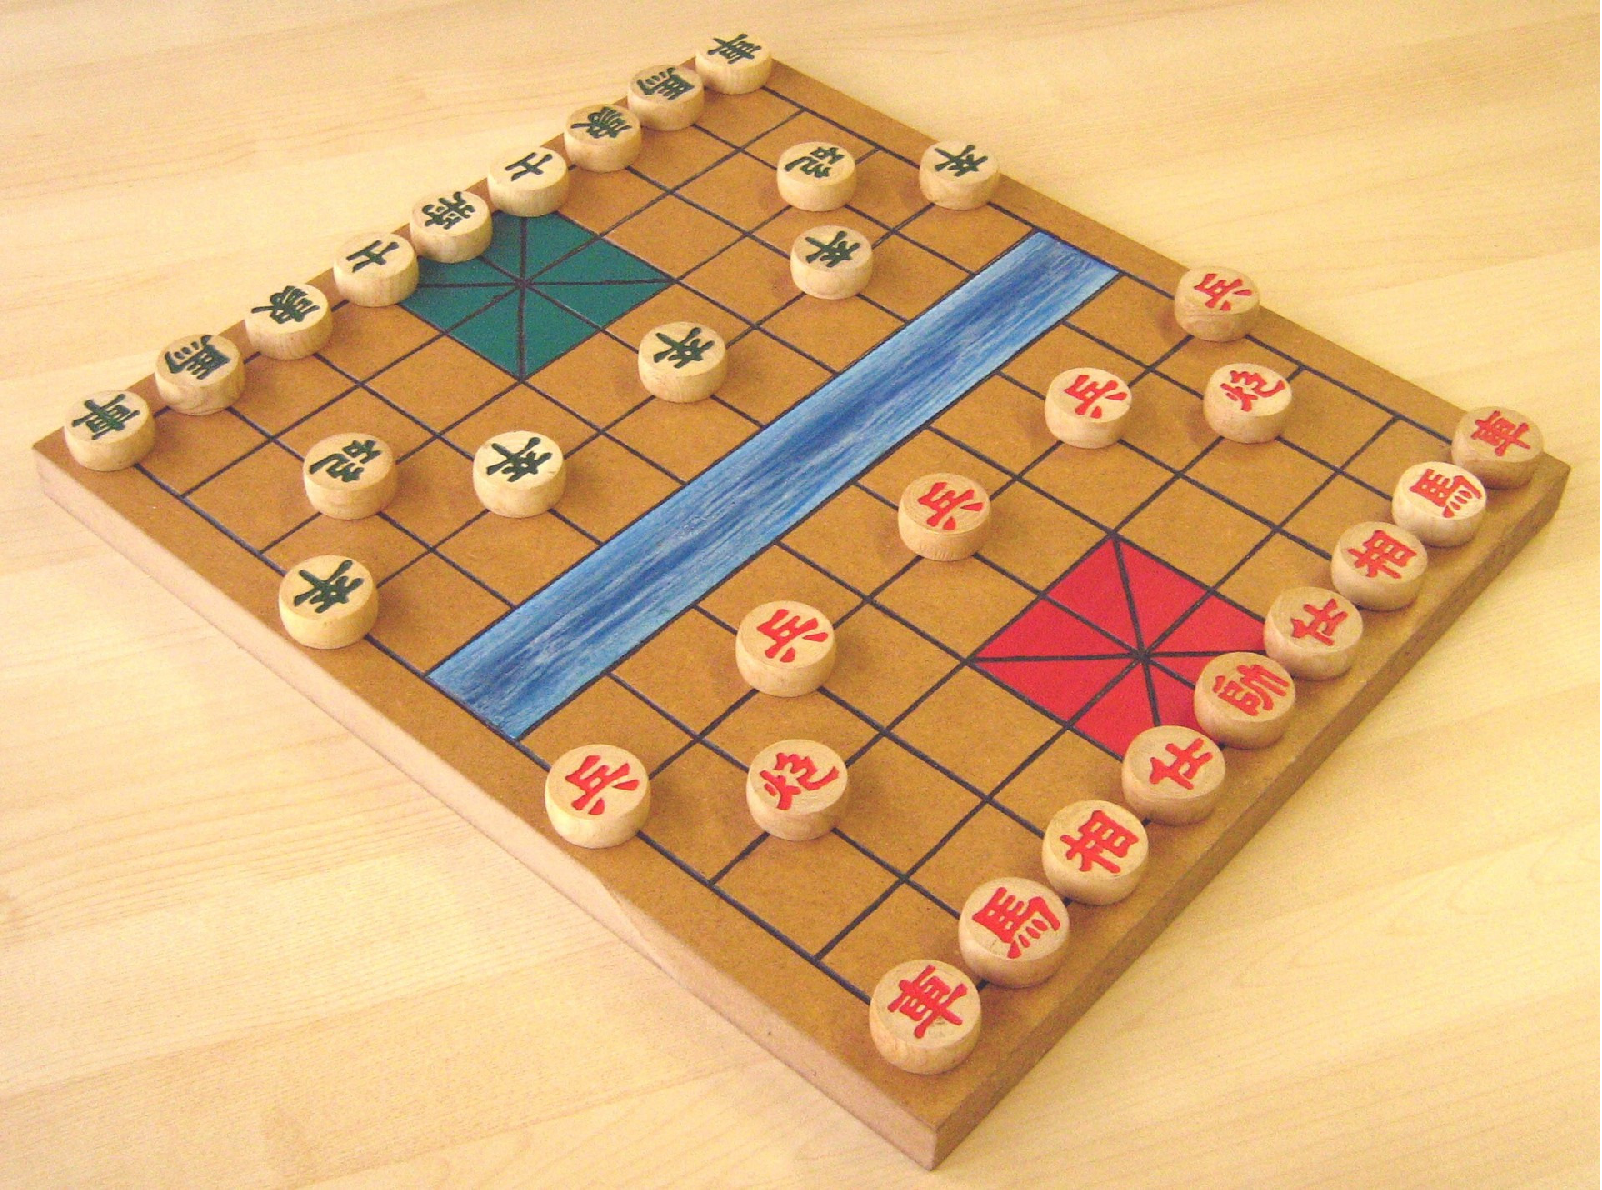
\includegraphics[width=0.7\textheight]{syanci}
            Сянци
        \end{figure}
    \end{columns}
\end{frame}
\note{%
    Для возможности быстро ощупать все фигуры, я использовал идеи
    восточно--азиатских аналогов европейских шахмат. В сёги (слева) и сянци
    (справа) фигуры имеют форму плоско--параллельной пластинки. Использование
    такой формы позволит не бояться зацепить какую-нибудь фигуру при движении
    рукой по доске.

    Так же это позволит упростить изготовление фигур.
}

\begin{frame}
    \frametitle{Замена штырьков на углубления в доске}
    \begin{figure}[htpb]
        \centering
        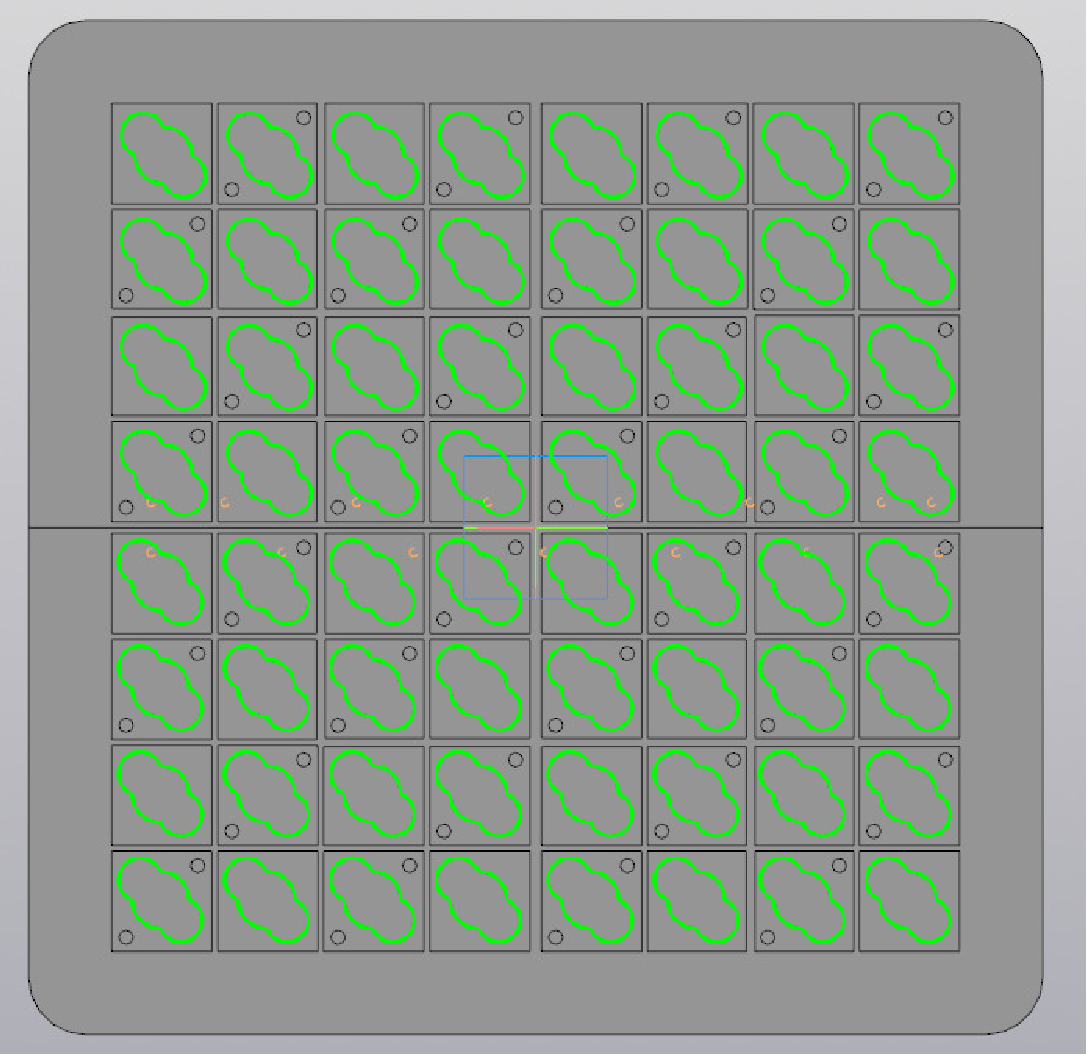
\includegraphics[height=0.8\textheight]{shtir}
    \end{figure}
\end{frame}
\note{%
    Для упрощения изготовления я отказался от штырьков в нижней части шахматной
    фигуры и вместо небольших отверстий, вырезать углубления, в которые будут
    вставляться фигуры. Так же это позволит увеличить надёжность фигур, так как
    штырьки не будут ломаться.
    \medskip%

    Для упрощения изготовления шахмат, я сделал клетки разного цвета на одном
    уровне, но для различия между ними, я на чёрных квадратах в левом нижнем и
    правом верхнем углах относительно игрока сделал небольшие углубления.
    \medskip

    Для упрощения ориентации игрока по полю, толщина прутьев, разделяющих
    клетки поля, сделана не равномерной.
}

\begin{frame}
    \frametitle{Нижняя часть доски}
    \begin{figure}[htpb]
        \centering
        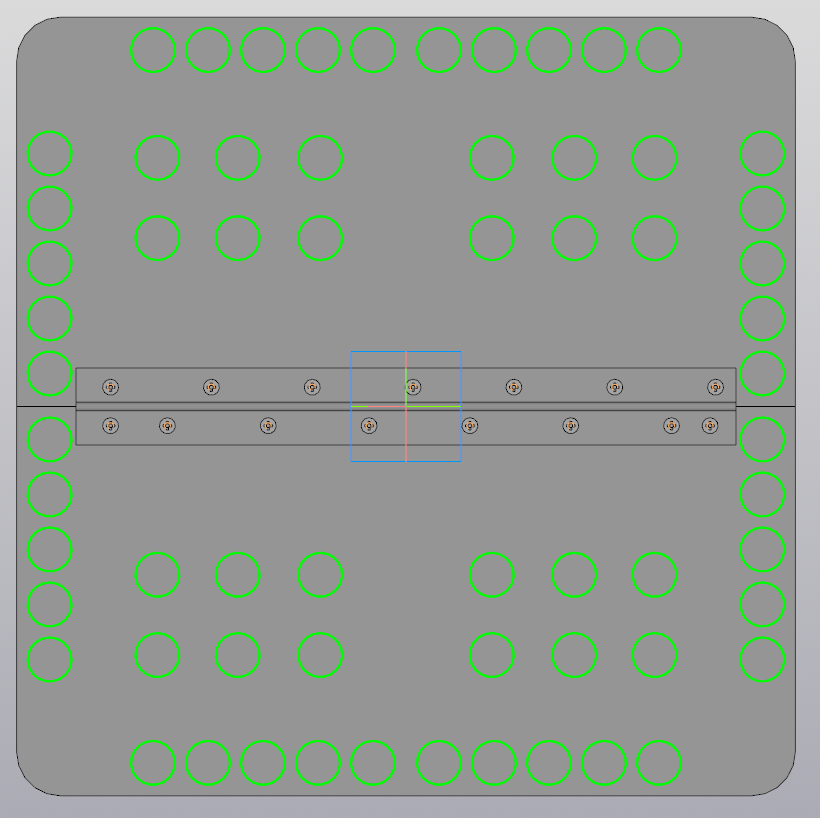
\includegraphics[height=0.8\textheight]{dno}
    \end{figure}
\end{frame}
\note{%
    Для упрощения складывания и раскладывания фигур, я отказался от обычно
    используемой полости в нижней части шахматной доски. Вместо неё были
    сделаны углубления в доске, в которых должны храниться фигуры. Так же, при
    систематическом складывании фигур, это сильно упростит раскладывание фигур.
}

\begin{frame}
    \frametitle{Шахматная фигура}
    \begin{figure}[htpb]
        \centering
        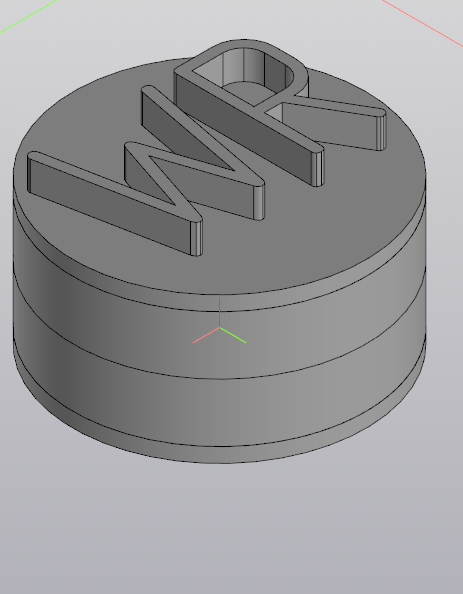
\includegraphics[height=0.8\textheight]{figur}
    \end{figure}
\end{frame}
\note{%
    Во избежание возможной путаницы, я отказался от использования шрифта
    Брайля. За место него было принято решение печатать названия фигур
    привычными буквами. Это так же позволит играть за такой доской и хорошо
    видящим людям. В качестве варианта нотации была выбрана английская нотация,
    так как она позволяет назвать любую фигуру лишь одной буквой. В качестве
    шаблона для названия фигуры был выбран шаблон вида цвет название.
}

\section{Практический этап}

\begin{frame}
    \frametitle{Реклама}
    \begin{figure}[htpb]
        \centering
        
\includegraphics[height=0.8\textheight]{adversting}
    \end{figure}
\end{frame}

\section{Заключение}

\begin{frame}
    \frametitle{Экономическая справка}
    \begin{center}
        {\tiny
        \begin{tabular}{p{1em} p{6em} p{6em} p{9em} p{8em} p{3em}}
            \toprule
             & На\-и\-ме\-но\-ва\-ние & Стоимость единицы материала & Единица материала &
                Ко\-ли\-чес\-тво единиц материала & Итого \\\midrule
            1 & Фанера & 292 & Лист 600 * 900 мм & 2 & 584 \\\midrule
            2 & ABS--пластмасса & 1200 & Килограмм & 0.064 & 77 \\\midrule
            3 & Петля & 20 & Штука & 2 & 40 \\\midrule
            4 & Саморез Шуц & 1 & Штука & 8 & 8 \\\midrule
            5 & Лак & 300 & Килограмм & 0.023 & 7 \\\midrule
            6 & Клей & 2'000 & Килограмм & 0.02 & 40 \\\midrule
            7 & Зарплата рабочего & 250 & Час & 2 & 500 \\\midrule
            \multicolumn{5}{l}{Себестоимость} & 1256 \\
            \bottomrule
        \end{tabular}
        }
    \end{center}
\end{frame}
\note{%
    С экономической точки зрения, проект успешен, так как его себестоимость
    всего в 1256 рублей. При рыночной цене шахматных наборов для слепых
    колеблющейся от 4990 до 9040 рублей, прибыль на продажу одного своего
    шахматного набора за половину от минимальной рыночной цены, то есть
    приблизительно 2500 рублей, составит 1244 рублей.

    Проектная работа выполнена успешно. Согласно целым проекта, была
    разработана и создан шахматный набор, удовлетворяющий моим требованиям.

    За время выполнения проекта, я улучшил своё мастерство в пользовании Vim,
    \LaTeX\, больше узнал о правилах составления документации.
}

\section*{}
\frame{\titlepage}
\end{document}
